\subsection*{Level 2}
The velocity controller from Exercise 3 was used as controller.
Following the first part of the task the chosen values can be seen in
Table~\ref{tbl:table2}.

\begin{table}[H]
  \centering
    \caption{Values for the velocity controller}
    \begin{tabular}{| c | c |}
		\hline
		Am & 500 \\ \hline
		$Ao_1$ & 1000 \\ \hline
		$Ao_2$ & 2000 \\
		\hline
    \end{tabular}
    \label{tbl:table2}
\end{table}

\subsubsection*{1}
Figure \ref{fig:task3_1_1000} shows the step responses for two different
values of $A_o$. A force of 5000 N is applied at the time 0.03 seconds.

\begin{figure}[H]
    \centering
    \begin{subfigure}[b]{0.45\textwidth}
        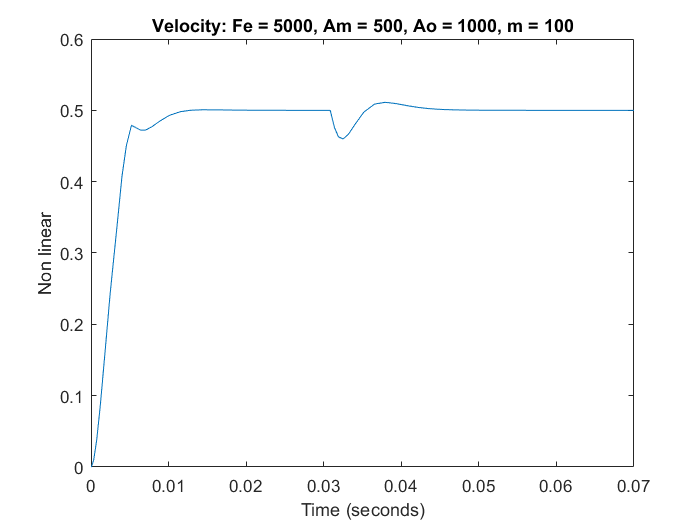
\includegraphics[width=\linewidth]{task3_1_1000.png}
    \end{subfigure}
    \begin{subfigure}[b]{0.45\textwidth}
        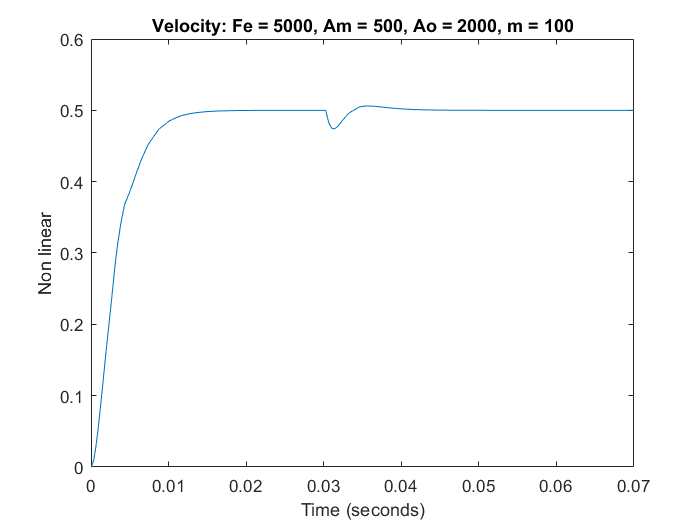
\includegraphics[width=\linewidth]{task3_1_2000.png}
    \end{subfigure}
	\caption{Comparison between the two different $A_o$ Values}
	\label{fig:task3_1_1000}
\end{figure}

\subsubsection*{2}
Figure \ref{fig:task3_2_1000} shows the step responses for two different
values of $A_o$ and now with a mass of 200 kg instead of 100 kg. The system
behaves more or less the same as with a mass of 100 kg.

\begin{figure}[H]
    \centering
    \begin{subfigure}[b]{0.45\textwidth}
        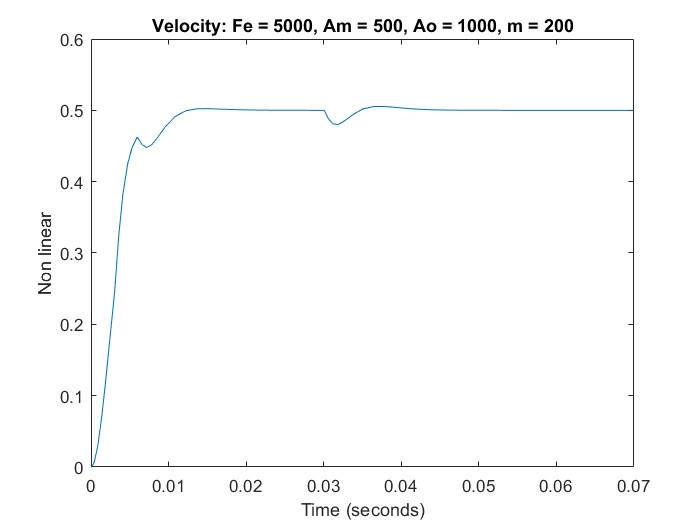
\includegraphics[width=\textwidth]{task3_2_1000.png}
    \end{subfigure}
    \begin{subfigure}[b]{0.45\textwidth}
        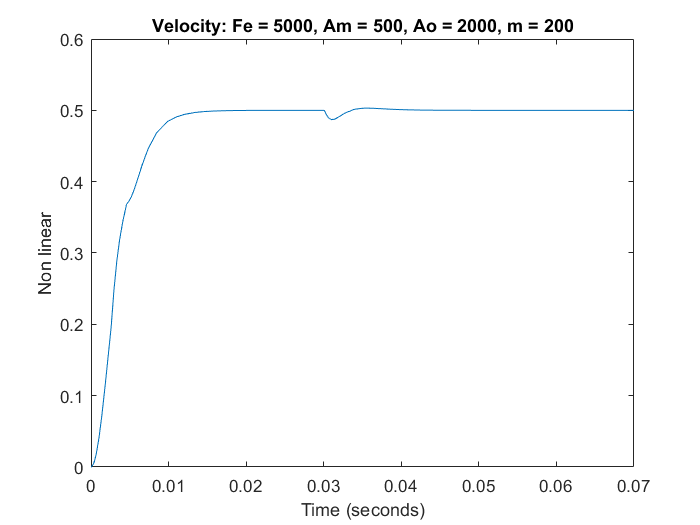
\includegraphics[width=\textwidth]{task3_2_2000.png}
    \end{subfigure}
	\caption{Comparison between the two different $A_o$ values}
	\label{fig:task3_2_1000}
\end{figure}

\subsubsection*{3}

Figure \ref{fig:task3_3_1000_freq_1700} shows the step responses for two
different values of $A_o$ with a sine wave as noise. The sine wave has a
frequency of 1700 rad/s.

\begin{figure}[H]
    \centering
    \begin{subfigure}[b]{0.45\textwidth}
        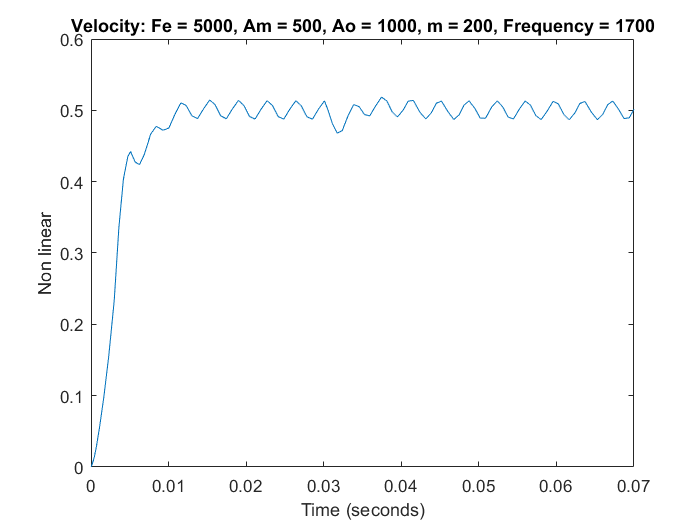
\includegraphics[width=\textwidth]{task3_3_1000_freq_1700.png}
    \end{subfigure}
    \begin{subfigure}[b]{0.45\textwidth}
        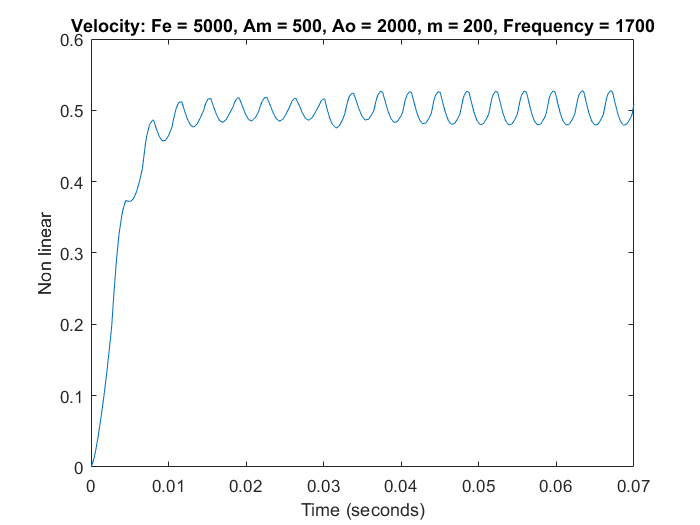
\includegraphics[width=\textwidth]{task3_3_2000_freq_1700.png}
    \end{subfigure}
	\caption{Comparison between the two different $A_o$ values}
	\label{fig:task3_3_1000_freq_1700}
\end{figure}

Figure \ref{fig:task3_3_bode} shows the complementary sensitivity
function for the two different $A_o$ values. The magnitude when the
frequency is 1700 rad/s is shown which shows that a lower $A_o$ value
dampens the noise more. It was hard to find a frequency were the noise
dampening were very noticeable but the dampening can be seen in Figure
\ref{fig:task3_3_1000_freq_1700} were the noise affects the system less
when $A_o$=1000 compared to $A_o$=2000.

\begin{figure}[H]
	\begin{center}
	
		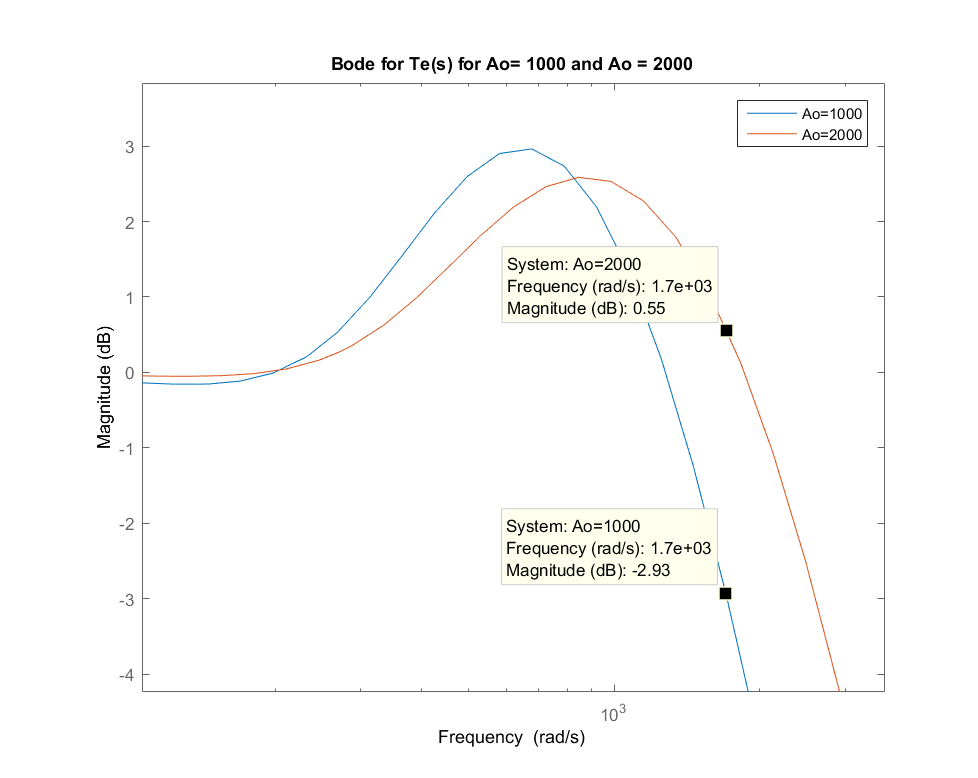
\includegraphics[width=0.45\linewidth]{task3_3_bode.png}
		\caption{Comparison between the complementary sensitivity functions}
		\label{fig:task3_3_bode}
	\end{center}
\end{figure}


%\end{document}
